\chapter{Balancing semilocal and nonlocal correlation}\label{chap:xc-functionals}

{\sffamily\mathversion{sans} This chapter presents a numerical analysis of the general range-separation approach between KS-DFT and vdW methods that served as a basis for Chapter~\ref{chap:vdw-methods}.
It shows that even though the effective range of semilocal XC functionals is not known explicitly, meaningful information about it can be obtained from the dependence of the DFT+vdW energies on the range-separating parameters of the vdW methods.
This approach rationalizes the choice of the underlying XC functional in a DFT+vdW method, which enables unbiased development of new vdW models---the topic of Chapter~\ref{chap:polarizability}.
The analysis stands on a large number of DFT and vdW calculations performed with different programs that are documented in detail in a public git repository~\citep{GitRepo}.
}

\section{Ambiguity in range separation}

As discussed in Section~\ref{sec:range-separation}, the DFT+vdW approach is based on the range separation of the XC energy, where a semilocal or hybrid KS-DFT and a vdW method cover the short- and long-range parts of the XC energy, respectively.
In nonmetals, the exchange energy is short-ranged and the long-range XC energy consists only of the correlation energy.
The rest of Chapter~\ref{chap:vdw-methods} then reviewed different methods for the long-range correlation energy, in most of which the range-separation is explicitly built-in via some distance-dependent function.
But as is clear from the brief exposition in Section~\ref{sec:xc-func}, the range-separation is not explicit in semilocal (hybrid) XC functionals (there is no sense of interelectronic distance in them), but is an implicit and relatively uncontrolled result of their construction and of the general shape of atomic and molecular densities.
As a result, the range-separating functions of the vdW methods cannot be guided theoretically by the behavior of the semilocal functionals, but become essentially empirical ``damping'' functions, whose parameters are fitted to reproduce accurate binding energies or other derived properties when combined with a particular semilocal functional.

In equilibrium, the contribution to the interaction energy of both the KS-DFT and the vdW parts are substantial in most systems, and the empirical approach to the range separation results in a state where it is not clear if a particular success (or failure) of a particular DFT+vdW combination is a result of the semilocal functional, the vdW method, or the system-dependent compatibility between the effective ranges of the two.
In an attempt to shed light on this problem, this chapter presents a detailed numerical study of the interplay between the short-range and long-range contributions to the XC energy on a large spectrum of systems.
The central part of the analysis is concerned with the dependence of the errors in binding energies of different DFT+vdW combinations on the respective range-separation parameters of the vdW models.

\section{Choice of tested methods and systems}

To get as much insight as possible from a numerical analysis, we selected a broad range of semilocal (hybrid) functionals, vdW methods and vdW-bound systems.
The XC functionals studied in this work span first four rungs of the ``Jacob's ladder of density functionals''~\cite{PerdewACP01}.
The first rung is occupied by a single functional, the LDA\@.
Although binding curves calculated with the LDA have incorrect asymptotic behavior and decay too fast, as expected from a local functional, equilibrium binding energies of vdW systems are usually strongly overestimated by LDA\@.
This spurious binding is not caused by the correlation part of LDA, but by the exchange part.
This feature is then shared in smaller degree by the next three rungs of the Jacob's ladder as well.
Whereas the HF exchange energy is always a repulsive contribution to the noncovalent interaction energy, many semilocal XC functionals bind noncovalent systems to a certain, usually insufficient degree via their exchange part.
This is caused by the implicit cancellation of errors between exchange and correlation in KS-DFT, and is reflected in the fact that most of the literature on the topic of vdW interactions and XC functionals is concerned with exchange, not correlation functionals~\cite{ZhangJCP97,PengPRX16}.

The second rung covers the GGA functionals.
It has been in this class of functionals, where most of the search for semilocal functionals with an ``appropriate'' XC range has been done, and mostly within the context of the vdW-DF nonlocal functional, because of the difficulties with the adaptation of its effective range.
Several special-purpose functionals designed to combine well with long-range correlation models were developed, ranging from completely new constructions~\cite{PernalPRL09,WellendorffPRB12}, to recombinations of older forms~\cite{CooperPRB10,HamadaPRB14,BerlandPRB14}, to simple reparameterizations of standard functionals~\cite{ZhangPRL98,KlimesJPCM10,KlimesPRB11}.
(An ``ideal'' exchange functional in this regard would be different from the exact exchange, because it would still contain a part of the short-range post-HF correlation that is not covered by GGA correlation functionals.)
All of these functionals perform well for vdW-bound systems (when combined with a vdW model), but not much is known about their accuracy for other systems, preventing them from becoming general methods.
Here, we test the most popular general-purpose GGA functional, PBE\@.

\begin{figure}[t]
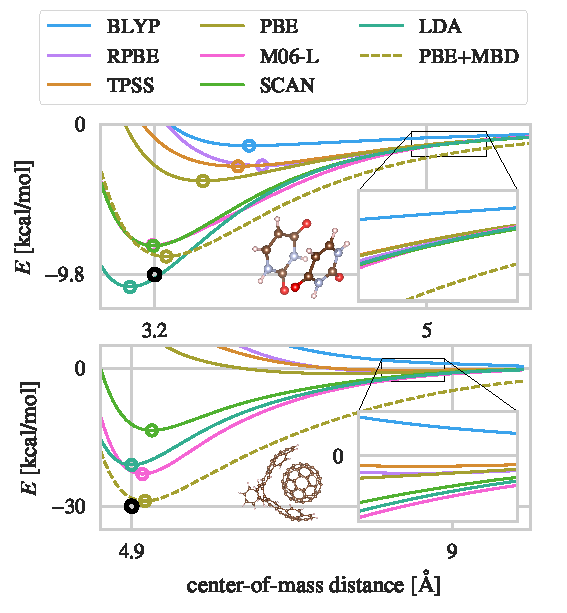
\includegraphics[center]{media/range-curves}
\caption{\textbf{Range of functionals.}
Binding energy curves of a stacked uracil dimer (top) and a C$_{60}$--buckycatcher complex (bottom) with different XC functionals.
The circles denote minima, the black circle corresponds to a reference value (see text).
PBE+MBD is shown as an example of a method with the correct (algebraic) asymptotic behavior.
}\label{fig:range}
\end{figure}

In the context of vdW interactions, considerably less attention has been paid to the to the third rung, the meta-GGA functionals, from which we include two functionals in our study.
The meta-GGA of \citet*{TaoPRL03} (TPSS) shares many aspects in its construction with the PBE functional, and also behaves similarly in description of noncovalent systems.
In contrast, the ``strongly constrained and appropriately normed'' (SCAN) functional of \citet{SunPRL15} is a substantial departure from PBE\@.
It is a recent development, which is intended to replace PBE for all purposes, with promising results across a broad range of systems in chemistry and physics, in many cases reaching the accuracy of hybrid functionals at a fraction of their computational cost~\cite{SunNC16}.
SCAN is still only a semilocal functional, however, and does not describe long-range electron correlation, resulting in a lack of long-range vdW interactions, as illustrated in Figure~\ref{fig:range}.

The fourth rung of functionals contains GGAs and meta-GGAs with partial admixture of exact exchange.
As in the HF method, exact exchange does not contribute to the vdW attraction at any distance, but substantially improves accuracy of (meta-)GGAs for many chemical problems. % chktex 36
Here, we study the hybrid GGAs PBE0~\cite{PerdewJCP96,AdamoJCP99} and B3LYP~\cite{BeckeJCP93}.
We also analyze SCAN0~\cite{HuiJCP16}, a PBE0-like version of SCAN with 25\% of exact exchange.
We do not include the fifth-rung functionals, such as the random-phase approximation or double-hybrid functionals, because they already contain long-range electron correlation by construction, at the price of much increased computational cost.

We chose three vdW methods to pair with the semilocal functionals, motivated by the following idea.
The semilocal functionals do not have an effective built-in range, but if a particular DFT+vdW is accurate and general, it can be said that the range of the XC functional must be complementary to that of the particular parametrization of the vdW model.
Hence, the vdW models, for which the effective range is known explicitly through their range-separation functions, can serve as a probe of the range of the XC functionals.
However, since the range separation in these effective models (both semilocal XC and vdW) is certainly not isotropic and is system dependent, judging the effective range from a single vdW method could lead to a bias.
To avoid this potential issue, we chose three vdW models with sufficiently different damping mechanisms.

In MBD (Section~\ref{sec:mbd}), the range-separation is controlled by a single sigmoid-shape damping function in~\eqref{eq:damping-ts}, whose range is controlled via a single parameter, $B\equiv\beta^\text{MBD}$, $A=6$, that determines at which fraction of a distance that is a sum of vdW radii of two atoms is the dipole potential damped to 50\%.
In the VV10 nonlocal functional (Section~\ref{sec:vdwdf}), the parameter $D=3^\frac23\pi^\frac56b^\text{VV10}/2$ in \eqref{eq:damping-vv10} controls the rate at which the effective resonance frequency of the local dipole response at two points increases (and hence polarizability decreases) as the points get closer to each other.
Both MBD and VV10 are functionals of the electron density, and likewise, the damping mechanism is density-dependent.
In contrast, the D3 method (Section~\ref{sec:pairwise}) depends only on the local geometry of the atomic structure around each atom, and unlike in MBD the atomic vdW radii are fixed and do not depend on the electron density.
The particular form of damping in D3 received some attention~\cite{GrimmeJCC11,SchroderJCTC15,SmithJPCL16,WitteJCTC17}, and of the two main variants (both based on atomic vdW radii), the original one is similar to that used in MBD, whereas the other, originally from \citet{JohnsonJCP06} (BJ), has a different limiting behavior at short range.
Since our goal here is to cover a broad range of vdW models, we use the BJ damping for its distinction from the damping used in MBD\@.
The BJ-damped D3 method uses three parameters that control its short-range behavior: $s_8^\text{D3}$ controls global mixing of the dipole--quadrupole term (which is inherently short-ranged due to its faster algebraic decay compared to the dipole--dipole term), and the closely related $a_1^\text{D3}$ and $a_2^\text{D3}$ control the onset of the dipole--dipole term ($a_1^\text{D3}$ scales vdW radii, $a_2^\text{D3}$ offsets them).

Whereas the vdW models have an explicit correlation range, the range of semilocal density functionals is only implicit, and the combined DFT+vdW models are therefore constructed by optimizing the range separation in vdW models against some benchmark properties, usually binding or lattice energies.
Several benchmark sets of vdW-bound systems have been established, of which we use predominantly three: the S66 set of 66 smaller organic dimers~\cite{RezacJCTC11}, the X23 set of 23 molecular crystals~\cite{Otero-de-la-RozaJCP12,ReillyJCP13}, and the S12L set of 12 large supramolecular complexes~\cite{GrimmeCEJ12}.
The S66 set is especially useful here, because each of the 66 dimers is given at 8 intermolecular distances distributed around the equilibrium distance, enabling at least partial separation of the short- and long-range behavior of a method.

Here, we shortly discuss only the expected accuracy of the reference values in the benchmark sets, and refer the reader to the cited works for additional details.
The S66 set was benchmarked with the coupled-cluster method with single, double, and perturbative triple excitations at the complete basis-set limit (CCSD(T)/CBS), a method that has been itself benchmarked to give at least an order-of-magnitude more accurate binding energies than any of the DFT+vdW methods investigated here~\cite{RezacJCTC13}. % chktex 36
The X23 benchmark lattice energies were obtained from experimental sublimation enthalpies by subtracting the zero-point vibration energy, with the estimated uncertainty of 1\,kcal/mol.
This was recently confirmed by CCSD(T) calculations of the benzene crystal (13.4\,kcal/mol compared to the benchmark value of 12.4\,kcal/mol)~\cite{YangS14}. % chktex 36
The S12L reference binding energies were obtained by subtracting calculated solvation and zero-point energies from experimental free energies of association.
Such a procedure has inherent uncertainty of several kcal/mol, which is supported by recent accurate diffusion quantum Monte Carlo calculations of the C$_{70}$--buckycatcher complex ($30\pm1$\,kcal/mol compared to the benchmark value of 27.5\,kcal/mol)~\cite{ZenPRB16}.

\section{Basis-set convergence of meta-GGA functionals}

\begin{table}[t]
\caption{\textbf{Dependence of PBE and SCAN binding energies (kcal/mol) of parallel-stacked uracil dimer on the basis-set size.}}\label{tab:basis-sets}
\mathversion{sans}
\begin{tabular}{lrrrr}
\toprule
& \multicolumn{2}{c}{PBE} & \multicolumn{2}{c}{SCAN} \\
basis set$^\text{a}$ & $\Delta_\text{CP}$ $^\text{b}$ & $E_\text{int}^\text{(CP)}$ $^\text{c}$ & $\Delta_\text{CP}$ & $E_\text{int}^\text{(CP)}$ \\
\midrule
cc-pVDZ       & $3.54$  & $-2.07$ & $2.88$  & $-7.07$ \\
cc-pVTZ       & $1.42$  & $-2.63$ & $1.12$  & $-7.82$ \\
cc-pVQZ       & $0.62$  & $-2.72$ & $0.43$  & $-7.93$ \\
aug-cc-pVDZ   & $0.96$  & $-2.70$ & $1.02$  & $-7.97$ \\
aug-cc-pVTZ   & $0.51$  & $-2.75$ & $0.54$  & $-7.97$ \\
aug-cc-pVQZ   & $0.07$  & $-2.76$ & $0.00$ & $-7.98$ \\
tight         & $0.18$  & $-2.69$ & $1.19$  & $-7.92$ \\
really\_tight & $0.19$  & $-2.68$ & $0.90$  & $-7.92$ \\
tight+tier-4       & $-0.29$ & $-2.77$ & $-0.17$ & $-7.99$ \\
\bottomrule
\end{tabular}

\small
$^\text{a}$``(aug)-cc-pV$X$Z'' are the correlation-consistent $X$-zeta basis sets of \citet{DunningJCP89}, the ``tight'' basis sets are the default sets of the FHI-aims program \citep{BlumCPC09}, ``+tier-4'' denotes the addition of all available basis functions.
$^\text{b}$Difference between the counterpoise corrected and uncorrected binding energies.
$^\text{c}$Counterpoise corrected binding energy.
\end{table}

Before delving in the analysis, we shortly discuss the issue of converging the KS-DFT binding energies with respect to basis-set size.
Table~\ref{tab:basis-sets} shows the binding energy of stacked uracil dimer (Figure~\ref{fig:range}) calculated with the PBE and SCAN functionals, with and without counterpoise correction, and with several different basis sets.
With the correlation-consistent basis sets of \citet{DunningJCP89}, the rate of convergence of both the PBE and SCAN functionals is similar.
With counterpoise correction, anything better than cc-pVDZ has acceptable accuracy ($\sim$0.2\,kcal/mol), and without counterpoise correction, only aug-cc-pVQZ gives such level of accuracy.
On the other hand, the numerical basis sets of FHI-aims give sufficient accuracy for PBE without counterpoise correction already on the ``tight'' level, which is an order of magnitude smaller than aug-cc-pvQZ\@.
Yet for SCAN, the ``tight'' level without counterpoise correction is insufficient, and only addition of the diffuse functions from the tier-4 group leads to converged binding energies.
The use of the ``tight'' basis set leads to systematic overbinding of all vdW bound systems.
This behavior is shared by the M06 family of meta-GGA functionals, but not by the TPSS functional.
Taking into account the results presented below, the slow convergence of the binding energy can be associated with meta-GGA functionals that take advantage of the abnormal behavior of the density in density-tail overlaps (small density, small reduced gradient, large electron delocalization function) to bind vdW systems more strongly in equilibrium.

\section{Range-separation on benchmark datasets}

The performance of approximate DFT+vdW methods on a given benchmark dataset is evaluated by comparing calculated binding energies, $E_i$, to the reference values, $E_i^\text{ref}$, yielding a distribution of errors, $\Delta E_i=E_i-E_i^\text{ref}$.
Since the interaction energies in vdW systems span orders of magnitude, we use relative errors, $\Delta_\mathrm rE_i=\Delta E_i/(-E_i^\text{ref})$ (assuming $E_i$ are negative).
The comparison of error distributions between different methods and systems is aided by introducing various statistical measures.
Two popular measures are the mean absolute error (MAE), $\sum_i\lvert\Delta E_i\rvert/N$, and mean absolute relative error (MARE), $\sum_i\lvert\Delta_\mathrm rE_i\rvert/N$, which both individually serve well as a single numerical indicator of performance, but do not provide much insight into the actual error distributions.
Instead, we use the mean relative error (MRE), $\sum_i\Delta_\mathrm rE_i/N$, and the standard deviation of the relative errors (SDRE),
\[ \text{SDRE}=\frac1N\sqrt{\sum_i(\Delta_\mathrm rE_i-\text{MRE})^2} \]
This enables us to study both the systematic error of a method (overall underbinding or overbinding), represented by MRE, as well as the ``statistical'' error (how consistent a method is in terms of the range of errors), represented by SDRE\@.

\begin{figure*}[t]
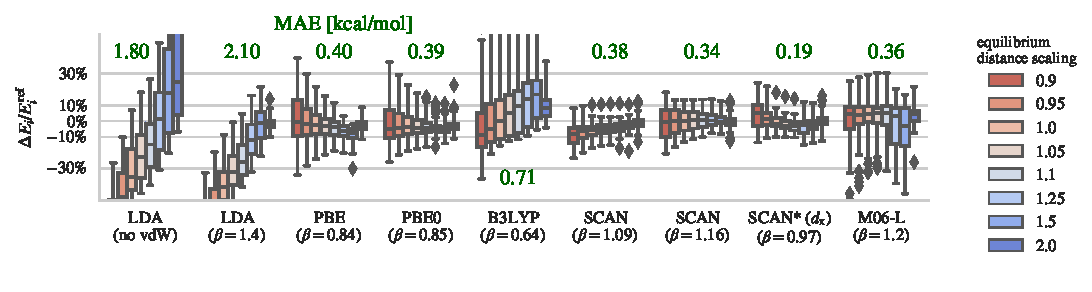
\includegraphics[center,width=0.95\linewidth]{media/s66-dists}
\caption{\textbf{Distributions of relative errors in binding energies on the S66 set of several DFT+MBD combinations.}
The distributions are displayed as box-and-whisker plots: a box shows the quartiles and whiskers represent the rest of the distribution, except for outliers that are more than 2.5-fold the interquartile distance from the box, which are shown individually.
The $x$-axis labels denote the functional and the value of the MBD range-separation parameter, $\beta^\text{MBD}$.
The blue--red spectrum encodes the scaling, $q$, of the respective equilibrium distances of individual complexes.
The green numbers indicate the mean absolute error (kcal/mol) for $q=1$.
The values of $\beta^\text{MBD}$ were selected as follows: $\beta$-values shown for PBE, PBE0, B3LYP, SCAN* (see text), and M06-L optimize MARE around $q=1$; $\beta=1.4$ for LDA optimizes MARE for $q=2$; and for SCAN and all $q$, $\beta=1.09$ optimizes SDRE, and $\beta=1.16$ optimizes MRE\@.
}\label{fig:s66-dists}
\end{figure*}

To study the range of the density functionals LDA, PBE, TPSS, SCAN, PBE0, B3LYP, SCAN0, and M06-L, we evaluated their combinations with the vdW methods MBD, VV10, and D3 at a range of their respective range-separation parameters, on the benchmark sets S66, X23, S12L, and other sets not discussed in this text.
We present a subset of these results below in Figures~\ref{fig:s66-dists} and~\ref{fig:param-fitting}, while the full data, obtained with FHI-aims~\cite{BlumCPC09} and Quantum Espresso~\cite{GiannozziJPCM09,HamannPRB13}, as well as computational details and other resources, are shared via a Git repository~\cite{GitRepo}.

The case of the S66 set and different DFT+MBD combinations (Figure~\ref{fig:s66-dists}) shows that summarizing the error distributions into a single number such as the mean absolute error reduces the method comparison to a one-dimensional classification, whereas comparing the full distributions in fact reveals distinct patterns specific to individual functionals.
Of the tested functionals, LDA is the only one that systematically overbinds S66 at equilibrium even without any long-range correction.
At the same time, when the equilibrium distances are scaled by 2, LDA predicts essentially no binding.
In this regard, although LDA binds vdW systems in equilibrium (too) strongly, it is very short-ranged.
The tail behavior can be fixed accurately by MBD with $\beta^\text{MBD}=1.4$, but the short-range overbinding cannot be compensated by a vdW energy term.
The increased overestimation of the XC energy with decreased distance then leads to the well-known underestimation of binding distances by LDA\@.
Already LDA thus illustrates that the degree to which a (semi-)local functional binds vdW systems is in general not a good measure for how well-suited it is for a generally applicable DFT+vdW method. % chktex 36

In contrast, both PBE and PBE0 are strongly underbinding S66 at all intermolecular separations, but with MBD and appropriate range separation ($\beta^\text{MBD}\approx0.83$), the resulting PBE+MBD and PBE0+MBD methods are well balanced, with symmetric error distributions, MAE independent of distance, and SDRE monotonously increasing at shorter distances.
The admixture of exact exchange decreases SDRE from 10.2\% with PBE to 8.7\% with PBE0 at equilibrium, but in general has only a small effect.
Another hybrid GGA, B3LYP, behaves as a true opposite of LDA, being at the same time very repulsive, yet quite long-ranged.
Even with a fairly short-range correlation covered by MBD ($\beta^\text{MBD}\approx0.7$), B3LYP+MBD still underbinds at equilibrium, and perhaps more surprisingly at longer distances.
In contrast to PBE/PBE0, the distributions are highly asymmetric, with underbound outliers being mostly the hydrogen-bonded complexes.

With SCAN, optimizing for MRE and SDRE leads to somewhat different values of $\beta^\text{MBD}$, 1.09 and 1.16, respectively, and correspondingly different error distribution profiles.
Both of these $\beta$ values are substantially larger than that for PBE, demonstrating the potentially longer range of SCAN\@.
When SDRE is optimized, SCAN+MBD has consistently narrower error distributions compared to PBE+MBD across all distances, with a slight systematic overbinding that grows with decreasing distances.
When MRE is optimized, the profile of SCAN+MBD is similar to that of PBE+MBD, with smaller outliers.
Adding exact exchange in SCAN0 (not shown) has even smaller effect than in PBE0, making the SCAN and SCAN0 error distributions almost indistinguishable.

Finally, M06-L requires only slightly larger amount of long-range correlation than SCAN, and most of the complexes from the S66 set are described well around equilibrium.
But several outliers are strongly overbound, and all complexes are overbound at longer distances, which is in line with previous studies~\cite{GoerigkJPCL15}.
Both issues may stem from the fact that the heavily fitted M06-L is parametrized also on the S22 set, a smaller version of S66, but S66 contains additional complexes and out-of-equilibrium complexes for which M06-L was not ``trained''.

\begin{figure*}
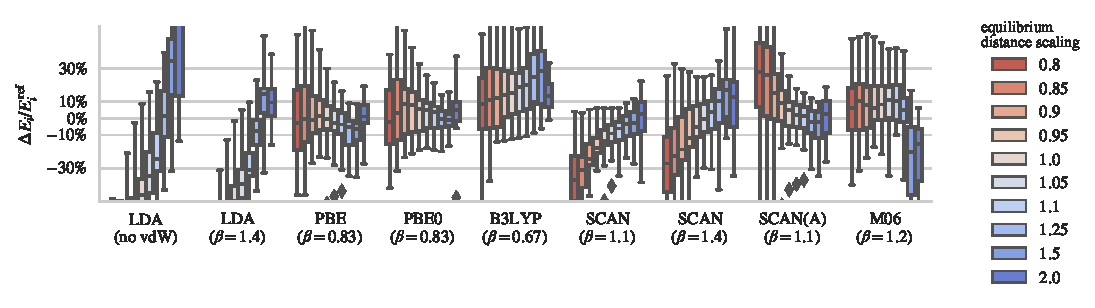
\includegraphics[center,width=0.95\linewidth]{media/x40-dists}
\caption{\textbf{Distributions of relative errors in binding energies on the X40 set of several DFT+MBD combinations.}
}\label{fig:x40-dists}
See Figure~\ref{fig:s66-dists} for caption.
\end{figure*}

To test the universality of the observations on the S66 set, we have repeated the same analysis for the X40 set of dimers of small halogenated hydrocarbons (Figure~\ref{fig:x40-dists}).
The overall errors are larger, because of the difficulty of modeling the polarizability of atoms with large partial charge, however, the general trends are similar to those found on the S66 set.

\begin{figure*}[t]
\makebox[\textwidth][c]{
\begin{tikzpicture}
% \node[below right, anchor=base] at (-2.5,-0.5) {{\ }};
\node[below right, anchor=base] at (0.5,-0.5) {{\bfseries a}};
\node[below right] at (0,0) {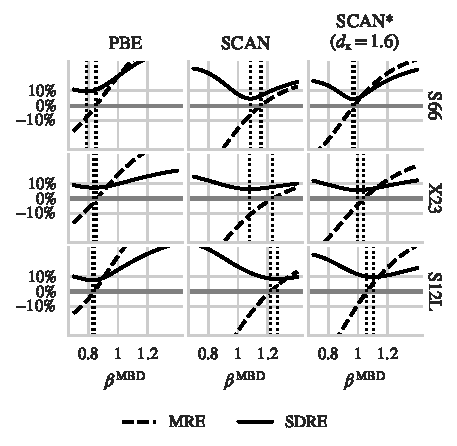
\includegraphics{media/mbd-param-fitting.pdf}};
\node[below right, anchor=base] at (8.1,-0.5) {{\bfseries b}};
\node[below right] at (7.6,-0.3) {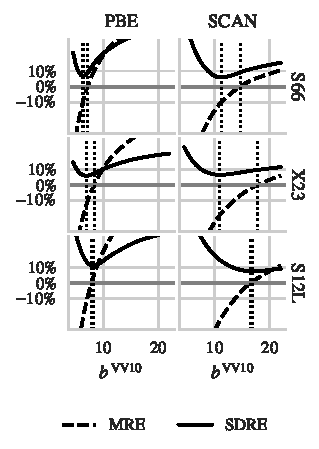
\includegraphics{media/vv10-param-fitting.pdf}};
\node[below right, anchor=base] at (13.6,-0.5) {{\bfseries c}};
\node[below right] at (13.1,-0.3) {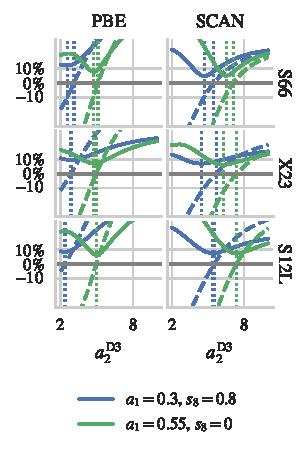
\includegraphics{media/d3-param-fitting.pdf}};
\node[below right, anchor=base] at (21,-0.5) {{\ }};
\end{tikzpicture}
}
\caption{\textbf{Dependence of means (MRE) and standard deviations (SDRE) of relative errors in binding energies on range-separation parameters.}
Three long-range correlation models with their respective parameters are shown: (\textbf a) MBD with $\beta^\text{MBD}$, (\textbf b) VV10 with $b^\text{VV10}$, and (\textbf c) D3 with $a_2^\text{D3}$.
Density functionals correspond to columns, and benchmark sets to rows within each subplot.
Only the equilibrium-distance configurations of the S66 set are used.
SCAN* denotes two reparameterizations of the SCAN functional discussed in the text. % chktex 36
The vertical dotted lines show where MRE equals to zero or SDRE reaches minimum.
For DFT+D3, two choices are shown of the two other range-separation parameters in D3: $a_1^\text{D3}$ and $s_8^\text{D3}$.
}\label{fig:param-fitting}
\end{figure*}

\begin{table}
\caption{\textbf{Overall performance of DFT+MBD methods.}}\label{tab:statistics}
\mathversion{sans}
\begin{tabular}{lrrrrrrr}
\toprule
functional & \multicolumn3c{MARE$^\text{a}$} & \multicolumn3c{MRE$^\text{b}$} & $\beta^\text{MBD,c}$ \\
& S66 & X23 & S12L & S66 & X23 & S12L & \\
\midrule
    LDA & 32\%  & 21\%  & 12\%  & $-31$\%  & $-17$\%  & 0.1\%    & $\infty$ \\
  B3LYP & 15\%  & 8.0\% & 12\%  & 5.2\%    & $-2.4$\% & 2.5\%    & 0.64     \\
    PBE & 8.4\% & 6.1\% & 5.3\% & $-2.1$\% & $-2.6$\% & $-0.4$\% & 0.84     \\
   PBE0 & 7.6\% & 5.4\% & 6.5\% & $-1.1$\% & $-1.7$\% & $-4.4$\% & 0.85     \\
   SCAN & 4.8\% & 8.4\% & 11\%  & $-3.0$\% & $-7.7$\% & $-10$\%  & 1.12     \\
  M06-L & 9.2\% & 16\%  & 29\%  & 2.4\%    & $-16$\%  & $-28$\%  & 1.20     \\
\bottomrule
\end{tabular}

\small
$^\text{a}$Mean absolute relative error.
$^\text{b}$Mean relative error.
$^\text{c}$Range-separation parameter of MBD minimizing MARE\@.
\end{table}

Of the tested functionals, PBE and SCAN (or their hybrid versions) show a potential to work as general balanced DFT+vdW methods.
To rule out the possibility that this conclusion about the two functionals is specific to MBD, we studied how MRE and SDRE of their combinations with MBD, VV10, and D3 depend on the respective range-separation parameters (Figure~\ref{fig:param-fitting}).
Comparing the results for the S66 set shows that all three vdW models have similar behavior, including the increased ambiguity in optimizing either for SDRE or MRE on the X23 set in the case of SCAN\@.
It is the case even for D3, which is potentially more flexible when adapting to a functional thanks to its three parameters.
Furthermore, Figure~\ref{fig:param-fitting} shows that whereas the optimal range separation of the vdW models is shared across different system types for the PBE functional, this is not the case for SCAN, for which the XC range seems to grow with the system size.
All these observations are true for all three vdW models.
Summarized results for other functionals are presented in Table~\ref{tab:statistics}.

SCAN has been previously combined with VV10 by \citet{PengPRX16} and with D3 and VV10 by \citet{BrandenburgPRB16}.
The obtained optimal values of $b^\text{VV10}$ were 15.7 and 14.0, respectively, and optimal parametrization of D3 was found to be $s_8^\text{D3}=0$, $a_1^\text{D3}=0.54$ and $a_2^\text{D3}=5.4$.
From the results in Figure~\ref{fig:param-fitting}, this corresponds to an optimal MRE on S66 for SCAN+VV10 (but systematic overbinding on X23 and S12L), and to optimal statistical error (SDRE) for SCAN+D3, leading again to some degree of systematic overbinding.
\citet{BrandenburgPRB16} associated this tendency mainly with hydrogen-bonded systems, which is in line with the observed overbinding of various ice structures by SCAN (without any vdW correction)~\cite{ChenPRB16}.

\citet{PengPRX16} argued that shifting the range separation between a semilocal functional and a vdW model towards the latter is beneficial.
Such a shift could also avoid some of the problems that long-range correlation models need to deal with at short range, such as the quadrupole interaction.
Our results confirm that such a shift is indeed possible in principle, but with the caveat that the description of the intermediate range by the density functional must be balanced and independent of system size.

\section{Three-body interactions}

\begin{figure*}[t]
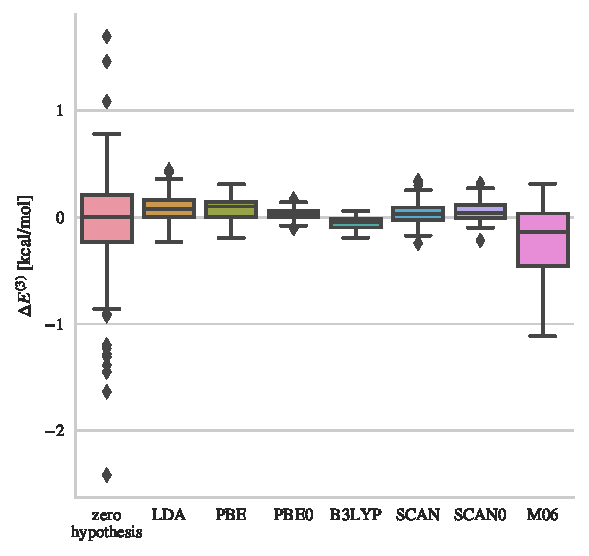
\includegraphics[center]{media/3-body}
\caption{\textbf{Distributions of relative errors in 3-body interaction energies on the 3B-69 set.}
The box-and-whisker plot is of the same kind as Figure~1 in the main text.
The ``zero hypothesis'' corresponds to a method which always gives zero 3-body interaction energy.
}\label{fig:3-body}
\end{figure*}

The total lattice energy of a molecular crystal can be decomposed into pairwise interactions between molecules, interactions between triples of molecules, etc.
Going up to four-body terms, \citet{YangS14} was able to calculate the lattice energy of the benzene crystal within the accuracy of 0.8\,kcal/mol.
Previously, \citet{TkatchenkoPRB08} found that many popular semilocal functionals overestimate the 3-body interaction energies in rare-gas dimers and crystals.

In the context of our present study, the 3B-69 dataset of 3-body interaction energies consists of three trimer structures from each molecular crystal from the X23 dataset~\cite{RezacJCTC15}.
In principle, this set could provide yet another independent (and more sensitive) measure of the range separation.
Interestingly, it turns out that the 3-body interaction energies are by far dominated by the short-range contribution from the semilocal functionals rather than the long-range 3-body terms, both with the many-body dispersion method as well as the 3-body correction of the D3 method.
Figure~\ref{fig:3-body} presents errors in the 3-body interaction energies of the 3B-69 set calculated with the semilocal functionals studied above.
Compared to a hypothetical method with zero 3-body interaction energies, most functionals give substantially better estimates, the only exception being M06.
However, the performance on the 3-body interactions does not seem to correlate with the performance for the total binding energies.
The LDA, PBE, and SCAN functionals perform comparably, whereas the B3LYP functional, which is relatively bad on the total binding energies gives very accurate 3-body interaction energies.

\section{System-size scaling}

\begin{figure}[t]
\makebox[\linewidth][c]{
\begin{tikzpicture}
\node[below right] at (1.1,.1) {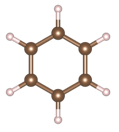
\includegraphics[height=1.2cm]{media/bz2.png}};
\node[below right] at (2.2,.1) {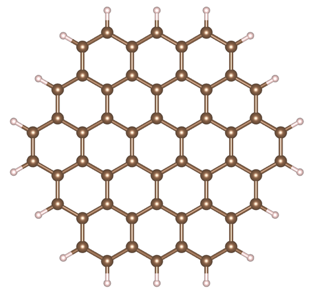
\includegraphics[height=1.2cm]{media/cor21.png}};
\node[below right] at (3.5,.1) {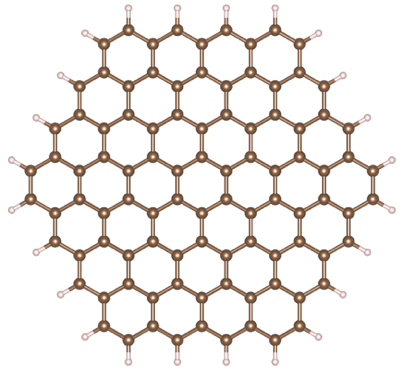
\includegraphics[height=1.2cm]{media/cor22.png}};
\node[below right] at (6.7,0) {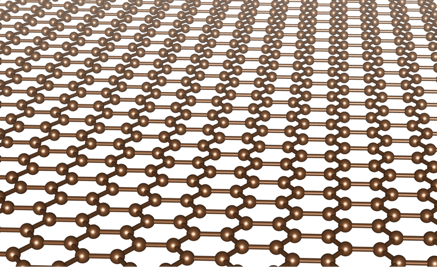
\includegraphics[height=1.0cm]{media/gr2.png}};
\node[below right] at (0,-1) {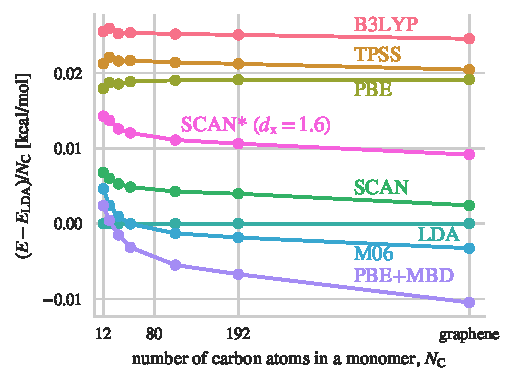
\includegraphics{media/flakes.pdf}};
\end{tikzpicture}
}
\caption{\textbf{Binding energies of graphene-flake dimers.}
The individual data points correspond to (increasing in size) benzene, naphtalene, pyrene, coronene, two larger circular hexagonal flakes (shown), and graphene.
All dimers are in a parallel-displaced configuration, as cut out from a graphite crystal without any geometry relaxations.
The plotted quantity is binding energy with respect to the LDA binding energy, per carbon atom.
The (infinite) number of atoms in graphene is set arbitrarily to 500.
}\label{fig:flakes}
\end{figure}

To gain further insight into the range of the functionals beyond statistical analysis, we calculated the binding energies of a series of graphene-flake dimers ranging from a benzene dimer to a graphene bilayer using DFT without any long-range correction (Figure~\ref{fig:flakes}).
We consider LDA as a reference short-range functional, accounting for any potential edge effects, and PBE+MBD as a reference full-range method.
The functionals B3LYP, PBE, and TPSS have a similar behavior to LDA, with the binding energies being offset only by a constant.
In contrast, the SCAN and M06 show a much stronger dependence on the system size, both at the small and large ends of the spectrum.
The difference in the offset to LDA between benzene dimer and graphene is 60\% for M06 and 35\% for SCAN with respect to PBE+MBD\@.
The ability to capture at least partially this system-size effect could be seen as advantageous, but it is unfortunate for developing DFT+vdW methods, because it breaks the core assumption that the functionals behave as short-range models of the electron correlation.
After all, these functionals are semilocal by construction and the fact that they are sensitive to this strongly nonlocal environment is contradicting this semilocality.
Furthermore, there are no known nontrivial exact constraints on the XC energy of overlapping density tails, and so the behavior of current semilocal functionals for such systems is essentially an uncontrolled result of the overall functional design, which complicates any development of ``farsighted'' density functionals.

Both SCAN and M06 are meta-GGAs, but so is TPSS, which does not show this sensitivity.
We speculate that in the case of SCAN, this sensitivity is caused by the particular parametrization of its dependence on the dimensionless electron localization parameter, $\alpha$.
SCAN uses the density parameter $\alpha$ in~\eqref{eq:scan-alpha} directly by interpolating and extrapolating forms constructed for $\alpha=0$ and $\alpha=1$, using the following function:
\begin{equation}
  f(\alpha)=\exp(-c_\mathrm{1x}\alpha/(1-\alpha))\theta(1-\alpha)
  -d_\mathrm x\exp(c_\mathrm{2x}/(1-\alpha))\theta(\alpha-1)
  \label{eq:scan-interp}
\end{equation}
where $\theta$ is the Heaviside step function, and $c_\mathrm{1x}=0.667$, $c_\mathrm{2x}=0.8$, and $d_\mathrm x=1.24$ are three of the total seven parameters in SCAN which are determined by fitting to properties (norms) of several model systems.
The values of $\alpha$ typically count in single figures within the electronic valence shells and decay slowly to zero with distance from the electronic system, while crossing $\alpha=1$ at some point~\cite{SunPRL13,BeckeJCP90}.
Among meta-GGA functionals, SCAN has a relatively wide plateau around $\alpha=1$ (due to Eq.~\ref{eq:scan-interp})~\cite{LoosJCP17}, where the enhancement factor, $F_\mathrm x$, is equal to 1, the value for the uniform electron gas.
This results in spatial regions in the electron density tails (dominated by HOMO, the highest-occupied molecular orbital) that are described with a uniform-like functional instead of the more appropriate single-orbital form of $\alpha\approx0$.
This can lead to sudden spikes in the exchange-correlation potential fairly outside the spatial regions where covalent bonding occurs~\cite{Gerit-private}.

\begin{figure}[t]
\centering
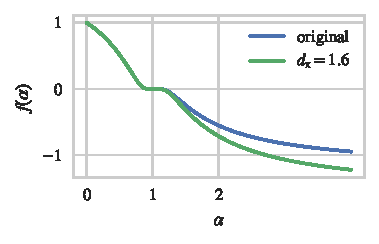
\includegraphics{media/scan-interp}
\caption{\textbf{Interpolation and extrapolation used in the SCAN exchange functional.}
The fixed points that are inter- and extrapolated are $\alpha=0$ and $\alpha=1$.
The shape of the function is controlled with three parameters, $c_\mathrm{1x}=0.667$, $c_\mathrm{2x}=0.8$, and $d_\mathrm x=1.24$ (original values).
}\label{fig:scan-interp}
\end{figure}

\section{SCAN reparametrizations}

In the series of graphene-flake dimers, the electronic gap (calculated with SCAN) decreases from 4.7\,eV for benzene dimer to 0.9\,eV for graphene bilayer, which makes the density tail decay slower with increasing system size.
Because the $\alpha=1$ behavior of SCAN makes it quite sensitive in the density tails, whose overlap also encodes the vdW bonding on the electron-density level, it only makes sense that SCAN is able to extract the nonlocal information about the system size via the decreasing electronic gap.
This mechanism could be also partially responsible for the discrepancies in optimal range separation for SCAN observed on the S66, X23, and S12L sets (Figure~\ref{fig:param-fitting}).

To check this hypothesis, we constructed several reparameterizations of SCAN and tested them on these benchmark sets.
We focused on the three parameters in Eq.~\ref{eq:scan-interp} because their values are determined weakly, having been fitted only to system-specific rather than universal norms.
We found that the overall XC range of SCAN can be changed substantially by modifying either of these parameters, without any regression in the overall performance of the SCAN+vdW methods.
However, the systems-size dependence of the optimal range separation for SCAN is not affected by either of them.
For illustration, Figures~\ref{fig:s66-dists},~\ref{fig:param-fitting}, and~\ref{fig:flakes} show results for a SCAN reparametrization with $d_\mathrm x$ changed from 1.24 to 1.6, which minimizes the overall error on S66 and reduces the XC range of SCAN (optimal $\beta^\text{MBD}$ of 0.97).
Figure~\ref{fig:flakes} clearly shows that the reparameterization does not change the sensitivity of SCAN in the density tails, as it only shifts the binding energy in graphene flakes by a constant.

Our toy reparameterization of the SCAN functional illustrates that the XC range of even a very sophisticated functional can be changed by a single parameter, whose value is not fixed by any physical constraint.
At the same time, it shows that a more subtle behavior of the XC range such as the system-size dependence is likely a result of the inherent functional form rather than a specific value of a numerical parameter.
Furthermore, we did not evaluate any other properties besides vdW binding, and it is quite possible that the new parameter values would introduce regressions for other systems.
To give a true alternative parametrization, the original fitting procedure would need to be performed with an additional constraint on vdW binding, perhaps expressed via a single simple system, which is beyond the scope of this work.
